\documentclass[conference]{IEEEtran}
\IEEEoverridecommandlockouts
\usepackage{cite}
\usepackage{amsmath,amssymb,amsfonts}
\usepackage{algorithm}
\usepackage{algorithmic}
\usepackage{graphicx}
\usepackage{textcomp}
\usepackage{xcolor}
\usepackage{booktabs}
\usepackage{url}
\usepackage{float}
\usepackage{tikz}
\usetikzlibrary{shapes,arrows,positioning,fit,backgrounds,calc,bending}
\usetikzlibrary{arrows.meta,shapes.geometric,decorations.pathreplacing}

\begin{document}

\title{Performance and Security Tradeoffs in Layered Authentication for Ephemeral Artificial Intelligence Agents}

\author{
\IEEEauthorblockN{Navin Suvarna*}
\IEEEauthorblockA{Independent Researcher\\
Holly Springs, NC, USA\\
nsuvarna@cisco.com\\
0009-0004-0161-2372\\
*Corresponding author}
\and
\IEEEauthorblockN{Karthik Pappu}
\IEEEauthorblockA{Dakota State University\\
Madison, SD, USA\\
karthik.pappu@trojans.dsu.edu\\
0009-0000-5335-6279}
\and
\IEEEauthorblockN{Saurabh Sharma}
\IEEEauthorblockA{Independent Researcher\\
Apex, NC, USA\\
saurabh.sharma24@gmail.com\\
0009-0001-5486-8062}
\and
\IEEEauthorblockN{Ankit Parashar}
\IEEEauthorblockA{Independent Researcher\\
Indianapolis, IN, USA\\
ankitparashar.ec.2110@gmail.com\\
0009-0008-6656-450X}
}

\maketitle

\begin{abstract}
Artificial intelligence agents increasingly act for users by spawning short-lived child agents that authenticate to internal services and terminate within seconds. OAuth offers two stronger mechanisms for such calls: token exchange, and sender-constrained proof-of-possession. Whether they are operationally justified for agent workloads has not been measured, since prior work addresses browser single sign-on and serverless identity rather than high-churn agents. We benchmark three authentication modes on a two-host testbed and evaluate them against five agent-specific threats.

The cost is small and, for realistic agent workloads, negligible: combining both mechanisms adds 3.85~ms over plain bearer tokens at the median, caching removes 65\% of that, and when the request performs an actual large-language-model call the entire authentication overhead is 0.8\% of end-to-end latency. Under sustained load the secure mode develops a bimodal tail, which we show is a queueing effect rather than a protocol limit: the tail falls in brief congestion episodes, the verifier stays flat throughout them, and one effective service time places the onset at the classical utilization knee. That yields a provisioning rule rather than a testbed-specific rate: keep per-worker utilization at or below 0.5, and jitter machine-paced arrivals.

The binding limits are compositional, not performance-related. Sender-constraining and audience scoping behave as specified at the resource server, yet delegation provenance is never recorded and fails silently, and a stolen token can be laundered through the exchange endpoint given client credentials. Practitioners should treat that endpoint, not the resource server, as the boundary determining what a layered deployment guarantees.
\end{abstract}

\begin{IEEEkeywords}
artificial intelligence agents, authentication, token exchange, proof-of-possession, OAuth 2.0, zero trust, tail latency, performance measurement, network services
\end{IEEEkeywords}

\section{Introduction}

\subsection{Problem Statement}

Artificial intelligence agents increasingly operate as autonomous software entities that invoke APIs, access protected resources, and act on behalf of users or upstream services. Unlike traditional web applications with persistent sessions or long-lived service identities, ephemeral AI agents may exist only for seconds or minutes, spawning and terminating rapidly in response to user requests, workflow orchestration, or resource constraints~\cite{authenticated_delegation_agents}.

This execution model creates a distinct authentication problem. Standard bearer-token patterns assume stable clients and accept some token-theft risk because tokens are time-bounded and tied to known clients~\cite{rfc6750,rfc9700}. Work on serverless and workflow-oriented access control shows that short-lived compute and dynamic invocation chains strain static IAM assumptions~\cite{sankaran2020,marin2022serverless}. Ephemeral agent environments intensify these concerns: although any individual token's exposure window is short, the aggregate attack surface expands and auditability is harder to preserve without explicit delegation metadata.

Layered authentication combines token exchange (RFC 8693~\cite{rfc8693}), sender-constrained tokens via proof-of-possession (RFC 9449~\cite{rfc9449}), and replay protection to narrow these exposure windows. However, existing OAuth security research has focused on formal analysis and implementation flaws in web SSO and service-provider deployments rather than on operational performance under high-churn agent workflows~\cite{oauth_formal,rahat2022cerberus}. Practitioners therefore lack empirical evidence on whether these mechanisms are operationally justified for ephemeral agents.

\textbf{Why AI agents differ from generic ephemeral microservices:} Three properties bear directly on authentication cost. Inter-arrival is bursty and chain-coupled, since an agent graph emits authenticated calls on Large Language Model (LLM) token cadence rather than user think-time. Backend latency is dominated by an external LLM call of typically 200--2000~ms, so tail variance matters more than absolute overhead. And delegation depth is variable, because an agent may spawn a subagent that spawns a tool-invoker, with accountability requiring the leaf token to carry the chain. Serverless functions and containers share short-lived identities but exhibit none of these; the mechanisms we evaluate apply to both, while the operational regime and threat model are agent-specific.

\subsection{Deployment Context}
\label{subsec:context}

The workload studied here is not hypothetical; it is what current agent-integration standards specify. The Model Context Protocol, which agent runtimes use to reach external tools, places a remote tool server in the OAuth~2.1 resource-server role and requires it to reject tokens not issued for it as audience. It also forbids token pass-through: a server calling an upstream API on the caller's behalf \emph{must} obtain a separate token rather than forward the one it received~\cite{mcp_authorization_2025}. That is precisely the audience-narrowing exchange evaluated here as Mode~B, and its short-lived-token guidance is what makes per-request rather than per-session cost the operationally relevant quantity.

The identity mechanisms are converging on the same shape. An active IETF draft treats agents as workloads requiring short-lived credentials bound to an agent identifier, chains authorization across domains by token exchange, and requires audit logs recording which delegated subject acted~\cite{kasselman2026aiagent}. A companion draft observes that actor context lacks a form surviving token transformation, and that inferring the actor from client identity breaks down when one client fronts many agents~\cite{mcguinness2026actor}. Those are the standards-side statement of T4 and T5; our measurements supply the empirical counterpart, since on a stock deployment the actor chain is not inconsistently represented but never recorded at all (\S\ref{subsec:rq3}).

\subsection{Research Questions}
Three research questions organize the study:
\begin{itemize}
\item \textbf{RQ1:} What latency and throughput overhead does layered authentication introduce for ephemeral artificial intelligence agents relative to a bearer-token baseline?

\item \textbf{RQ2:} How do token caching and agent churn affect the performance and reliability of layered authentication?

\item \textbf{RQ3:} What security gains are achieved by adding sender-constrained tokens and delegation-aware token exchange against replay, token theft, and audience misuse?
\end{itemize}

\subsection{Contributions}

\textbf{1. A utilization model for sender-constrained-token tail latency:} We identify a bimodal tail-latency regime in Mode~C emerging between 256 and 384 requests per second (RPS) on a single-worker verifier, and explain it. Per-request timing shows the tail is \emph{episodic}, concentrated in a few multi-second episodes through which throughput and the verifier stay flat. A single effective service time places the onset at the classical utilization knee and correctly predicts a four-worker configuration not used to calibrate it; a Poisson sweep at matched utilization isolates phase-coherent arrivals as a second condition. This yields two operator-measurable quantities and a provisioning rule rather than a testbed number.

\textbf{2. Agent-specific threat model, tested at both boundaries:} We refine the generic OAuth threat model to five agent-specific threats and realize each empirically rather than enumerating it abstractly. Four target the resource server; the fifth targets the token-exchange endpoint, and it is there that we find the layered guarantees stop: delegation provenance is silently never recorded, and a stolen sender-constrained token could be re-bound on the version studied.

\textbf{3. Empirical evaluation with pre-registered methodology:} A 195-run matrix over a two-host topology with injected RTTs of 0/1/10/50~ms and real LLM-backed workloads, using randomized run order, pre-registered outlier criteria, bootstrap 95\%~CIs and pairwise Mann-Whitney $U$ with Cliff's $\delta$.

\textbf{4. Reproducible artifact:} We release the prototype, realm configuration, analysis pipeline, attack harness and benchmark drivers, with every claim sourced from machine-readable JSON or CSV.

Section~\ref{sec:related} positions the work; Section~\ref{sec:model} states the threat model, modes and pre-registered metrics; Section~\ref{sec:method} describes the prototype and matrix; Section~\ref{sec:results} reports results; Section~\ref{sec:discussion} interprets them, states limitations and gives deployment guidance.

\section{Related Work}
\label{sec:related}

OAuth 2.0~\cite{rfc6749} established delegated authorization through limited-scope access tokens, and subsequent formal analyses clarified its security properties and deployment assumptions~\cite{oauth_formal,oidc_formal}. RFC 8693~\cite{rfc8693} extends the model with token exchange, enabling audience narrowing and delegation context across service hops, a direction also pursued through capability-oriented extensions for chained authorization~\cite{li2022capability}. Sender-constrained tokens address the residual weakness of bearer designs: RFC 9449~\cite{rfc9449} defines Demonstrating Proof of Possession (DPoP), which binds an access token to a client-held key, mitigating theft and replay at the application layer, and is more deployable in lightweight clients than certificate binding via mutual TLS~\cite{rfc8705}. Formal analysis of high-assurance profiles underscores the value of these defenses~\cite{fapi2_formal}, while empirical work keeps documenting weaknesses in real OAuth deployments~\cite{rahat2022cerberus}.

Adjacent work on workload identity, zero-trust microservices, and serverless security emphasizes short-lived identities and invocation-level authorization~\cite{eztrust2019,pontes2023spire,marin2022serverless,nist_zta}, with recent studies addressing agent-specific delegation~\cite{authenticated_delegation_agents,zouari2025leastprivilege}. None measures short-lived agent instances under high churn, the gap this paper addresses empirically.

\textbf{Position relative to baselines:} Two literatures are closest to this work and each leaves a measurable gap. The Financial-grade API (FAPI) 2.0 formal-analysis line~\cite{fapi2_formal,oauth_formal,oidc_formal} establishes correctness properties for sender-constrained-token profiles but reports no end-to-end latency, tail behavior, or per-component decomposition under operational network conditions. The serverless-IAM and workload-identity literature~\cite{sankaran2020,marin2022serverless,eztrust2019,pontes2023spire} measures cold-start and invocation-level overheads but treats authentication as one opaque cost rather than decomposing it into exchange, proof generation, verification and replay-cache stages. Our contribution sits at the intersection: statistically grounded measurement of the DPoP-bound exchange across a two-host stack with injected RTT bands, and a concurrency sweep that surfaces a Mode-C-specific bimodal tail onsetting between 256 and 384 RPS, which neither literature could observe by construction. As an anchor, the Keycloak project's tuned multi-node benchmarks report 2{,}000 logins/s and 10{,}000 token refreshes/s~\cite{keycloak2025bench}; our single-instance verifier surfaces the regime at a far lower 384~RPS.

\section{System Model and Problem Formulation}
\label{sec:model}

\subsection{Threat Model}
\label{subsec:threats}

Ephemeral agents complicate the bearer-token threat surface in four ways: they spawn other agents, creating delegation chains; they retry autonomously, creating replay surfaces across hops; they share infrastructure with agents of other principals, enabling audience misuse; and their identities are short-lived enough that audit pipelines built around long-lived users may miss intermediate actors. We refine the generic enumeration into five agent-specific threats, tested empirically and summarized in Fig.~\ref{fig:threats}:

\begin{figure}[htbp]
\centering
\resizebox{0.88\columnwidth}{!}{%
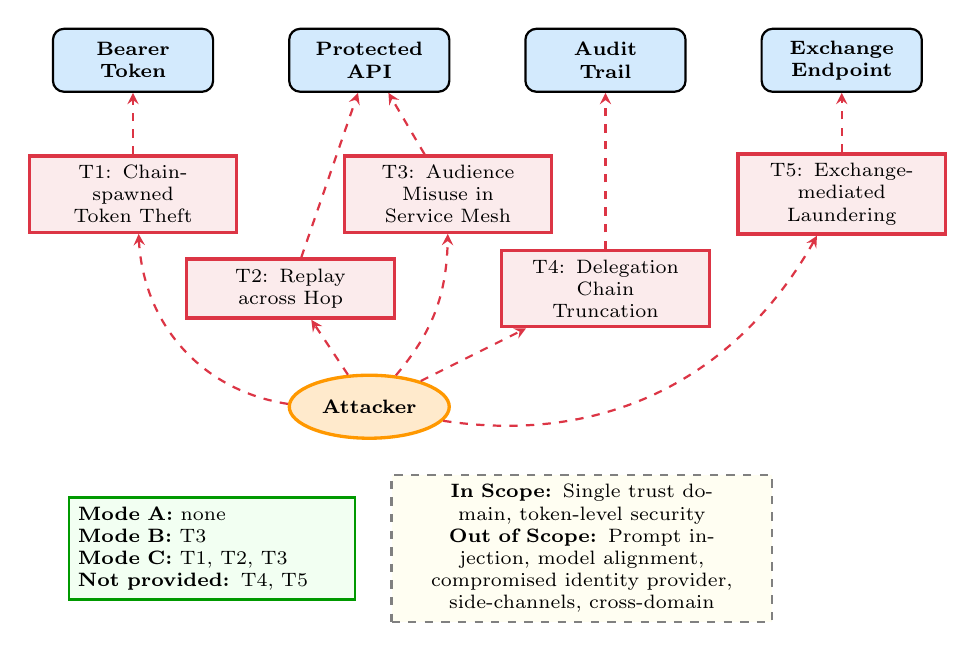
\begin{tikzpicture}[font=\scriptsize]

\definecolor{threatred}{RGB}{220,53,69}
\definecolor{assetblue}{RGB}{33,150,243}
\definecolor{attackorange}{RGB}{255,152,0}

\tikzset{
    asset/.style={
        rectangle, rounded corners,
        minimum width=1.8cm, minimum height=0.8cm,
        text width=1.8cm, align=center,
        draw=black, thick, fill=assetblue!20,
        font=\scriptsize\bfseries
    },
    threat/.style={
        rectangle,
        minimum height=0.75cm,
        text width=2.4cm, align=center,
        draw=threatred, very thick, fill=threatred!10,
        font=\scriptsize
    },
    attacker/.style={
        ellipse,
        minimum width=1.8cm, minimum height=0.8cm,
        text centered,
        draw=attackorange, very thick, fill=attackorange!20,
        font=\scriptsize\bfseries
    },
    noteleft/.style={
        rectangle,
        draw=green!60!black, thick, fill=green!5,
        text width=3.4cm, align=left,
        font=\scriptsize
    },
    notecenter/.style={
        rectangle,
        draw=gray, dashed, thick, fill=yellow!5,
        text width=4.6cm, align=center,
        font=\scriptsize
    },
    attack/.style={->, >=stealth, thick, draw=threatred, dashed}
}

% Assets
\node[asset] (token) at (-3.0,3.2) {Bearer\\Token};
\node[asset] (api)   at (0,3.2)    {Protected\\API};
\node[asset] (audit) at (3.0,3.2)  {Audit\\Trail};
\node[asset] (exch)  at (6.0,3.2)  {Exchange\\Endpoint};

% Threats — agent-specific (see Section III.A)
\node[threat] (t1) at (-3.0,1.5) {T1: Chain-\\spawned\\Token Theft};
\node[threat] (t2) at (-1.0,0.3) {T2: Replay\\across Hop};
\node[threat] (t3) at (1.0,1.5)  {T3: Audience\\Misuse in\\Service Mesh};
\node[threat] (t4) at (3.0,0.3)  {T4: Delegation\\Chain\\Truncation};
\node[threat] (t5) at (6.0,1.5)  {T5: Exchange-\\mediated\\Laundering};

% Attacker
\node[attacker] (attacker) at (0,-1.2) {Attacker};

% Attack paths
\draw[attack] (t1) -- (token);
\draw[attack] (t2) -- (api);
\draw[attack] (t3) -- (api);
\draw[attack] (t4) -- (audit);
\draw[attack] (t5) -- (exch);

\draw[attack] (attacker) to[bend left=40] (t1);
\draw[attack] (attacker) -- (t2);
\draw[attack] (attacker) to[bend right=20] (t3);
\draw[attack] (attacker) -- (t4);
\draw[attack] (attacker) to[bend right=35] (t5);

% Protection mechanisms
\node[noteleft] at (-2.0,-3.0) {
\textbf{Mode A:} none\\
\textbf{Mode B:} T3\\
\textbf{Mode C:} T1, T2, T3\\
\textbf{Not provided:} T4, T5
};

% Scope annotation
\node[notecenter] at (2.7,-3.0) {
\textbf{In Scope:} Single trust domain, token-level security\\
\textbf{Out of Scope:} Prompt injection, model alignment,\\
compromised identity provider,\\ side-channels, cross-domain
};

\end{tikzpicture}%
}
\caption{Agent-specific threat model. T1--T5 are realized empirically as S1--S4 and S6 (\S\ref{subsec:rq3}). Mode~C covers the widest surface at the resource server; T4 and T5 are addressed by no mode, since they arise where RFC~8693 composes with RFC~9449 and with its own delegation semantics, upstream of the verifier. Dashed arrows: attack paths from attacker through threat to asset.}
\label{fig:threats}
\end{figure}

\begin{enumerate}
\item \textbf{T1 (Chain-spawned token theft):} A parent agent spawns a child and delegates a token to it; on shared compute that token is exposed through memory, transient logs, or sidecar interception, and an attacker presents it from an unrelated network position. The distinction from familiar bearer-token theft is aggregate rather than per-token exposure: each leak window is brief, but the spawning topology multiplies the tokens in flight per task. Tested as~S1.

\item \textbf{T2 (Same-\texttt{jti} replay across a delegation hop):} A request traverses intermediaries such as a workflow router or tracing sidecar, any of which terminates TLS and can capture the complete request including its DPoP proof, then replay it. Tested as~S2.

\item \textbf{T3 (Audience misuse in a multi-tenant service mesh):} A token correctly scoped for one internal service is presented to another sharing the same authorization server, which weak audience binding permits~\cite{li2022capability,yang2023k8sperm}. The agent context sharpens this: each spawned agent typically calls exactly one service, so a mis-scoped token is an unambiguous violation. Tested as~S3.

\item \textbf{T4 (Delegation-chain truncation):} The \texttt{act} claim should record the intermediaries at depth two or greater. An attacker or buggy intermediary presents a truncated chain, so the request appears to originate at the parent and the accountability delegation should supply is defeated. Tested as~S4.

\item \textbf{T5 (Exchange-mediated laundering of a stolen token):} T1--T4 attack the resource server; T5 attacks the authorization server. A compromised sibling agent holds both another agent's token and the client credentials its own runtime requires. Rather than replaying the token where Mode~C's sender-constraint would reject it, the attacker presents it to the exchange endpoint as a \texttt{subject\_token}. Whether the constraint survives depends on the server checking \texttt{subject\_token}'s \texttt{cnf.jkt} against the key presenting the proof; if it does not, the protection is stripped one hop upstream of where it is enforced. Tested as~S6, scenario numbering follows test order, S5 (expired-token reuse) predating this taxonomy.
\end{enumerate}

\textbf{Attacker capabilities:} S1--S3 assume only \emph{captured request material}, a token or a token and its proof taken from memory, transient logs or a TLS-terminating intermediary, held by an attacker with no long-term secret. S6 additionally assumes \emph{client credentials}, realistic in precisely the topology T1 describes, since scraping a child agent's memory for its token generally yields the client secret beside it; S6a reports the weaker attacker separately. Throughout, the authorization server, verifier and primitives are assumed sound: we attack protocol composition, not implementations. Expired-token reuse (S5) is tested but sits outside the taxonomy as baseline hygiene. Out of scope: prompt injection and model alignment, compromised authorization servers, verifier side channels, and cross-domain federation.

\subsection{System Assumptions}

We assume a single trust domain with one trusted authorization server (Keycloak); a secure agent--API channel (TLS in production, simulated in the testbed); correct ECDSA, SHA-256 and JWT processing; and an available replay cache, whose degraded operation is also evaluated. An \textit{ephemeral agent} is a short-lived process spawned by an orchestrator that obtains tokens at creation, issues one or more API calls, and terminates within seconds to minutes. Agent \textit{churn} is the rate of agent creation per second; higher churn increases contention for issuance, replay-cache access and verification.

\subsection{Authentication Modes Under Study}

We compare three authentication modes.
\begin{enumerate}
\item \textbf{Mode A (Direct Bearer Token):}
The agent obtains an access token through the client-credentials grant and presents it to the API in the \texttt{Authorization} header. This mode performs no token exchange and uses no proof-of-possession.

\item \textbf{Mode B (Token Exchange Bearer):}
The agent first obtains an access token and then exchanges it for an audience-specific token using RFC 8693 token exchange. The exchanged token carries a narrowed audience and, where applicable, delegation metadata such as an actor chain. It remains a bearer token.

\item \textbf{Mode C (Token Exchange + Proof-of-Possession):}
Mode C extends Mode B by sender-constraining the exchanged token with DPoP. The agent generates an ECDSA P-256 key pair, includes a DPoP proof in the token-exchange request, and receives a token containing a \texttt{cnf.jkt} claim that binds the token to the public key. Each API request includes a DPoP proof JWT with \texttt{htm}, \texttt{htu}, \texttt{ath}, \texttt{jti}, and a signature. The API validates the proof and checks the replay cache.
\end{enumerate}

\subsection{Metrics and Hypotheses}
\label{subsec:metrics}

Four outcome categories are evaluated. For latency (RQ1) the primary endpoint is the median at the headline cell with a bootstrap 95\% CI, supported by P95/P99/max and per-stage decomposition across token exchange, JSON Web Key Set (JWKS) lookup, bearer decode, DPoP-signature verification and replay-cache access. For throughput (RQ2) it is sustained RPS without authentication failures, swept 32--512~RPS single-worker and extended to 2048~RPS with four workers. For security (RQ3) it is the HTTP status and error code in each adversarial scenario.

Four hypotheses were pre-registered before the two-host collection, with thresholds from an earlier single-host pilot and RFC~9449. \textbf{H1}, that uncached $\tilde{\ell}_C - \tilde{\ell}_A$ falls in $[5,10]$~ms with a large effect, is \emph{partially supported}: the effect is large ($\delta = 0.80$) but the gap is 3.85~ms, below the bound, because the two-host stack is faster than the pilot that set it. \textbf{H2} (caching cuts Mode~C's median $\ge$50\%, residual $\le 5$~ms) is \emph{supported} (65\%; 1.34~ms); \textbf{H3} (S1--S3 return their RFC-mandated rejections) is \emph{supported}; and \textbf{H4} (Mode~C's p95 becomes bimodal above a threshold rate while $\mathrm{p95}_B/\mathrm{p95}_A$ stays below 3$\times$) is \emph{supported}, bimodal at 384 and 512~RPS with ratio 1.94 at 512.

\section{Experimental Methodology}
\label{sec:method}

This is an applied experimental study (per Edgar and Manz, Ch.~8~\cite{edgar2017research}): a controlled prototype is used rather than a field deployment because repeatable manipulation of clock skew, RTT, arrival distribution, and cache state is infeasible against a production authorization server. The prototype reproduces RFC~6749/8693/9449 with production artifacts (Keycloak~26.2, Redis~7, ECDSA P-256, JWT). Findings are intended to inform single-domain agent deployments using a standards-compliant OAuth authorization server and a co-located replay cache; \S\ref{subsec:limits} bounds what does not follow from this scope.

\subsection{Prototype Architecture}
\label{subsec:prototype}

Figure~\ref{fig:architecture} summarizes the prototype. Keycloak~26.2 acts as the OAuth~2.0/OIDC authorization server with RFC~8693 exchange; a launcher spawns ephemeral agents at churn rates of 1, 5 or 20~agents/s; those agents act as short-lived clients under one of the three modes; a FastAPI protected API validates bearer tokens, DPoP proofs and audience claims; and Redis~7 serves as the TTL-based \texttt{jti} replay cache. The agent client is Python 3.11 using \texttt{httpx}, \texttt{PyJWT} and \texttt{cryptography} for ECDSA P-256; timing uses \texttt{time.perf\_counter()}.

\textbf{Two-host topology with same-host loopback variant:}
To expose operational network latency, Keycloak, its Postgres store and Redis run on a dedicated authorization-server host while the launcher, protected API and workload generator run on a separate client host, so the authorization server and replay cache are network-distant from the resource server. The headline RQ1 cell and the stress sweep are collected with infrastructure and API co-located on loopback, isolating authentication cost from network-stack variance; the netem sweep (Fig.~\ref{fig:netem}) re-injects RTT bands.

\textbf{Network latency injection:}
A two-host deployment alone does not yield interpretable RTT bands, so a netem sidecar sharing each infrastructure container's network namespace applies a \texttt{tc qdisc} rule that disappears with the sidecar. We sweep $\{0, 1, 10, 50\}$~ms (same-rack, same-AZ, intra-region, inter-region), three replications per mode and band, each a full sweep preceded by a discarded warm-up pass so session drift falls across replications rather than confounding delay ordering.

\textbf{Clock skew accommodation:}
Cross-host operation exposes clock skew. We measured a 69~s offset and accommodated it by widening three freshness windows: the bearer-token leeway, the DPoP-proof freshness check, and a forward shift on the proof's \texttt{iat}. NTP-synchronized deployments use tight defaults (10~s, 60~s, 0~s); the testbed values are recorded in the artifact and are not load-bearing below, except for S5 (\S\ref{subsec:rq3}).

\begin{figure}[htbp]
\centering
\resizebox{0.88\columnwidth}{!}{%
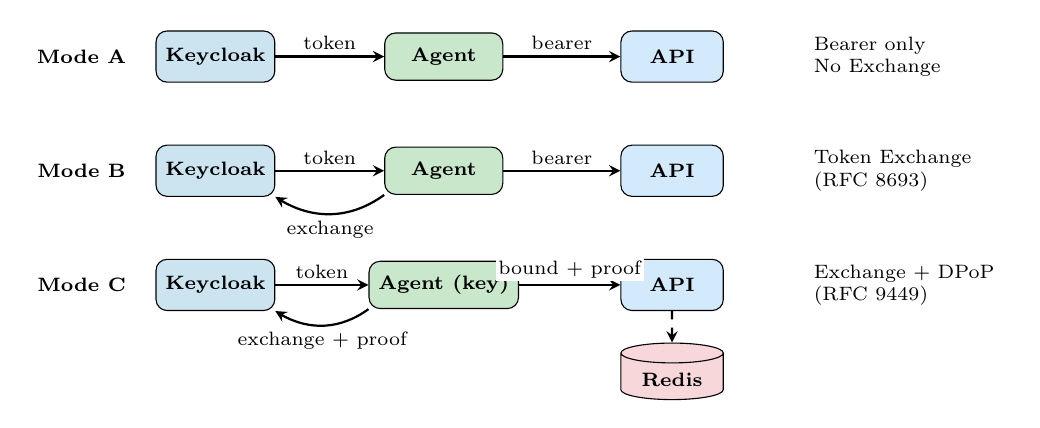
\begin{tikzpicture}[font=\scriptsize]

% Colors
\definecolor{keycloakblue}{RGB}{0,120,180}
\definecolor{agentgreen}{RGB}{76,175,80}
\definecolor{apiblue}{RGB}{33,150,243}
\definecolor{redisred}{RGB}{220,53,69}

% Styles
\tikzset{
    component/.style={
        rectangle, rounded corners,
        minimum width=1.5cm, minimum height=0.65cm,
        text centered, draw=black, fill=blue!10,
        font=\scriptsize\bfseries
    },
    agent/.style={
        rectangle, rounded corners,
        minimum width=1.5cm, minimum height=0.6cm,
        text centered, draw=black, fill=agentgreen!30,
        font=\scriptsize\bfseries
    },
    service/.style={
        rectangle, rounded corners,
        minimum width=1.3cm, minimum height=0.65cm,
        text centered, draw=black, fill=apiblue!20,
        font=\scriptsize\bfseries
    },
    storage/.style={
        cylinder, shape border rotate=90, aspect=0.25,
        minimum height=0.65cm, minimum width=1.3cm,
        draw=black, fill=redisred!20,
        font=\scriptsize\bfseries
    },
    arrow/.style={thick, ->, >=stealth},
    lbl/.style={font=\scriptsize, inner sep=1pt, fill=white},
    modelabel/.style={font=\scriptsize\bfseries},
    note/.style={font=\scriptsize, text width=2.4cm, align=left}
}

% ---------------- Mode A ----------------
\node[modelabel] at (-4.6,0.2) {Mode A};
\node[component, fill=keycloakblue!20] (kc_a) at (-2.9,0.2) {Keycloak};
\node[agent] (ag_a) at (0,0.2) {Agent};
\node[service] (api_a) at (2.9,0.2) {API};
\draw[arrow] (kc_a) -- node[lbl,above=1pt] {token} (ag_a);
\draw[arrow] (ag_a) -- node[lbl,above=1pt] {bearer} (api_a);
\node[note] at (5.9,0.2) {Bearer only\\No Exchange};

% ---------------- Mode B ----------------
\node[modelabel] at (-4.6,-1.25) {Mode B};
\node[component, fill=keycloakblue!20] (kc_b) at (-2.9,-1.25) {Keycloak};
\node[agent] (ag_b) at (0,-1.25) {Agent};
\node[service] (api_b) at (2.9,-1.25) {API};
\draw[arrow] (kc_b) -- node[lbl,above=1pt] {token} (ag_b);
\draw[arrow] (ag_b.south west) to[bend left=35] node[lbl,below=1pt] {exchange} (kc_b.south east);
\draw[arrow] (ag_b) -- node[lbl,above=1pt] {bearer} (api_b);
\node[note] at (5.9,-1.25) {Token Exchange\\(RFC 8693)};

% ---------------- Mode C ----------------
\node[modelabel] at (-4.6,-2.7) {Mode C};
\node[component, fill=keycloakblue!20] (kc_c) at (-2.9,-2.7) {Keycloak};
\node[agent] (ag_c) at (0,-2.7) {Agent (key)};
\node[service] (api_c) at (2.9,-2.7) {API};
\node[storage] (cache_c) at (2.9,-3.9) {Redis};
\draw[arrow] (kc_c) -- node[lbl,above=1pt] {token} (ag_c);
\draw[arrow] (ag_c.south west) to[bend left=35] node[lbl,below=1pt] {exchange + proof} (kc_c.south east);
\draw[arrow] (ag_c) -- node[lbl,above=1pt] {bound + proof} (api_c);
\draw[arrow, dashed] (api_c) -- (cache_c);
\node[note] at (5.9,-2.7) {Exchange + DPoP\\(RFC 9449)};

\end{tikzpicture}%
}
\caption{Per-mode architecture. Mode~A: one token grant, presented as a bearer. Mode~B: a second round trip exchanges it for an audience-scoped token (RFC~8693), still a bearer. Mode~C: the exchange carries a DPoP proof and returns a key-bound token; each API call carries a fresh proof (RFC~9449), and only this mode consults the \texttt{jti} replay cache (dashed).}
\label{fig:architecture}
\end{figure}

\subsection{Experiment Matrix}

The experiment matrix varies four factors:
\begin{enumerate}
    \item \textbf{Authentication mode:} A, B, and C.
    \item \textbf{Cache mode:} Off (fresh token and key per request) and On (token reuse within a 4-minute window and key reuse for the agent lifetime).
    \item \textbf{Agent churn:} 1, 5, and 20 agents/s.
    \item \textbf{Delegation depth:} 1-hop (no actor) and 2-hop (actor chain simulated via \texttt{actor\_token} in token exchange).
\end{enumerate}

This produces $3 \times 2 \times 3 \times 2 = 36$ conditions. We replicate each non-headline condition five times and the headline condition (cache-off, churn=5, depth=1) ten times per mode, yielding $33 \times 5 + 3 \times 10 = 195$ runs in total. The headline cell is replicated twice as often because it alone feeds the bootstrap CIs and pairwise tests of Table~\ref{tab:latency}. Run order is randomized by a seeded shuffle (seed \texttt{20260506}, persisted in \texttt{benchmark\_summary.csv}) so condition is decorrelated from execution time and the order is reproducible. The full RTT-sweep matrix multiplies by the four netem bands. The design is a census of the factor space rather than a sample from it: all 36 conditions are executed, so replication counts govern precision rather than coverage. At the headline cell the bootstrap CI half-width is 0.03--0.05~ms against a reported effect of 3.85~ms, so the design resolves differences well over an order of magnitude smaller than the one it reports.

\subsection{Measurement Procedure}

Each run starts containers, waits for health checks, executes a 10\,s warmup (excluded) and records for 60\,s. Per request we log mode, cache, churn, depth, status, latency, exchange and verification time, and replay/audience flags; LLM runs (\S\ref{subsec:realism}) add token counts and per-call latency. We report median and 95\%~bootstrap CIs of the median (10\,000 resamples, seed \texttt{20260506}); pairwise differences use Mann-Whitney $U$ (two-sided) and Cliff's $\delta$ with magnitude thresholds per Romano et al.~\cite{romano2006appropriate}. Requests within a run are not independent; treating each run's median as one observation ($n=10$ per mode) leaves the headline differences unchanged (3.89, 3.49 and 0.40~ms, each $p=1.8\times10^{-4}$).

Per-run exclusion follows a pre-registered policy (\texttt{OUTLIER\_POLICY.md}): a run is excluded if wall-clock duration exceeds $1.5\times$ target, failure rate is $>3\sigma$ above the per-condition mean (and $\ge 1$~pp absolute), replay cache is unavailable, or any container reports \texttt{unhealthy}. Exclusion is per-run not per-request (tail-latency observations are signal, not noise); replacements use seed+1 and both seeds are recorded.

\subsection{Realism: Synthetic vs.\ LLM-backed workloads}
\label{subsec:realism}

The headline numbers in \S\ref{subsec:rq1} use a synthetic no-op API handler, isolating authentication cost from backend variance as RQ1 requires. A realism condition issues a chat completion to an externally hosted LLM after the authenticated Mode~C call, with fixed 50--60-token prompts and a sliding-window budget guard ($\le$\,18\,K/min, $\le$\,720\,K/hr, $\le$\,4.75\,M/day). Across three replications at the headline cell ($n=776$, all HTTP~200), \emph{LLM} latency is 1376~ms median / 1735~ms P95, while Mode~C \emph{auth} cost on the same requests is 10.8~ms median / 19.4~ms P95, consistent with the synthetic baseline: $\approx$\,0.8\% of end-to-end median and $\approx$\,1.1\% at P95, an order of magnitude below the LLM's own tail variance.

\section{Results}
\label{sec:results}

\subsection{RQ1: Latency and Throughput Overhead}
\label{subsec:rq1}

Table~\ref{tab:latency} summarizes end-to-end latency at the headline cell (churn 5\,agents/s, depth~1, ten replications pooled to $n=3000$ per mode). Cache-off medians rise 6.12~$\to$~9.54~$\to$~9.97~ms across Modes~A, B, C; the B$\to$C increment reflects elliptic-curve proof generation, verification, and replay-cache lookup. Pairwise Mann-Whitney $U$ rejects equality at $p<10^{-100}$ for A-vs-B and A-vs-C and at $p=9.95\times 10^{-50}$ for B-vs-C; with Holm correction across the three comparisons ($m=3$) every adjusted $p$ remains below $10^{-49}$, so the family-wise error rate is controlled at $\alpha=0.05$ without altering any conclusion. Cliff's $\delta$ magnitudes are 0.77 for A-vs-B and 0.80 for A-vs-C (both \emph{large} per Romano et al.~\cite{romano2006appropriate}) but only 0.22 for B-vs-C (\emph{small}): the steady-state separation between Mode~B and Mode~C is real but modest; their operational distinction emerges in the tail under load (\S\ref{subsec:rq2}).

Caching (token reuse within validity window; Mode~C key reuse for agent lifetime) cuts Mode~C's median 65\% to 3.44~ms with a 1.34~ms residual over cached Mode~A (Table~\ref{tab:latency}).

\begin{table}[htbp]
\caption{End-to-end latency at the headline cell (churn 5/s, depth 1; $n=3000$ cache-off, $n=1500$ cache-on per mode). CI: bootstrap 95\% CI of the median (10\,000 resamples, seed 20260506); per-pair statistics in \texttt{significance\_tests.json}.}
\label{tab:latency}
\centering
\resizebox{\columnwidth}{!}{%
\begin{tabular}{lccccc}
\toprule
\textbf{Mode} & \textbf{Cache} & \textbf{Median (ms)} & \textbf{95\% CI} & \textbf{P95 (ms)} & \textbf{Overhead} \\
\midrule
A (Bearer) & Off & 6.12 & [6.09,~6.15] & 11.97 & --- \\
B (Exchange) & Off & 9.54 & [9.50,~9.60] & 15.93 & +3.42~ms \\
C (DPoP) & Off & 9.97 & [9.93,~10.03] & 17.33 & +3.85~ms \\
\midrule
A (Bearer) & On & 2.10 & [2.08,~2.11] & --- & --- \\
B (Exchange) & On & 2.10 & [2.09,~2.12] & --- & 0.00~ms \\
C (DPoP) & On & 3.44 & [3.41,~3.46] & --- & +1.34~ms \\
\bottomrule
\end{tabular}%
}
\end{table}

\textbf{Decomposition under injected RTT:}
Figure~\ref{fig:netem} sweeps netem-injected one-way delays of $\{0, 1, 10, 50\}$~ms across the authorization-server and replay-cache namespaces. Mode~A's median grows $\sim$1:1 with RTT (one round-trip), Mode~B $\sim$2:1 (token + exchange), Mode~C $\sim$4:1 (adding the DPoP-verifying cache lookup); at 50~ms Mode~C reaches median 235.9~ms / P95 255.0~ms. This separates network from cryptographic cost, which a single-host prototype cannot.

\begin{figure}[htbp]
\centering
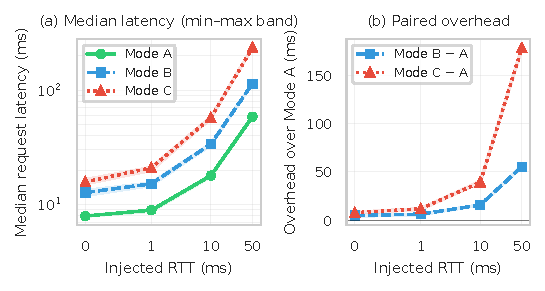
\includegraphics[width=\columnwidth]{figures/netem_rtt_sweep.pdf}
\caption{End-to-end latency at the headline cell vs injected RTT between agent host and infrastructure, three replications per mode and RTT band. Mode~A solid, Mode~B dashed, Mode~C dotted, for grayscale legibility. (a) Median of the per-run medians; the band spans their min--max across replications; y-axis log-scale. (b) Overhead differenced within each replication before aggregating. Mode~A scales $\sim$1$\times$ RTT (one round-trip), Mode~B $\sim$2$\times$ (token + exchange), Mode~C $\sim$4$\times$ (token + exchange + DPoP-verifying replay-cache lookup).}
\label{fig:netem}
\end{figure}

\textbf{Auth cost relative to the agent's own workload:}
The figures above isolate authentication; under the LLM-backed condition (\S\ref{subsec:realism}) the same Mode~C cost is \textbf{0.8\% of end-to-end median latency and 1.1\% at P95}, two orders of magnitude below the model call it protects. For agent workloads the tradeoff is, in absolute terms, close to free; what follows is about the conditions under which that stops being true.

\textbf{Key Finding (RQ1):} Mode~C adds 3.85~ms median over bearer-only ($\delta=0.80$, large); 65\% is absorbed by caching (1.34~ms residual); against a real LLM-backed request this is 0.8\% of end-to-end latency. Under injected RTT, overhead scales linearly with each mode's round-trip count, the regime characterized in \S\ref{subsec:interpret}.

\subsection{RQ2: Cache and Churn Effects}
\label{subsec:rq2}

Across the churn rates in the main matrix (1, 5 and 20 agents/s) every mode sustained 100\% success and linear throughput over all 195 runs and 98{,}101 requests. That range sits far below the verifier's saturation point. To locate the rate at which the interaction manifests, we swept all three modes at 32, 128, 256, 384 and 512 sustained RPS on the loopback configuration (\S\ref{subsec:prototype}) with netem cleared. To bypass the asyncio coordination ceiling of a single launcher process ($\approx$94~RPS), the generator was scaled into parallel workers (one per 64~RPS), each minting valid per-request DPoP proofs through the RQ1 client. Replication was concentrated where variance mattered (Table~\ref{tab:stress}, column $n$). Across $\sim$417{,}000 requests every cell returned 200, with no \texttt{proof not active} or \texttt{replay\_attack} rejection (Table~\ref{tab:stress}).

\begin{table}[htbp]
\caption{Side-by-side stress sweep, authorization-server loopback, $n$ replications per cell at 30\,s record each, no netem, 100\% success. The p95 column reports the median p95 across replications, so a wide min--max bracket reflects dispersion across replications rather than within one run. Bolded cells mark the bimodal Mode-C cells (384 and 512 RPS).}
\label{tab:stress}
\centering
\resizebox{\columnwidth}{!}{%
\begin{tabular}{lrrrrr}
\toprule
\textbf{Mode} & \textbf{Agg.\ RPS} & \textbf{$n$} & \textbf{Median (ms)} & \textbf{p95 (ms; median [min--max])} & \textbf{Max (ms)} \\
\midrule
A & 32  & 2  & 5.94  & 11.62 & 164 \\
A & 128 & 2  & 5.28  & 8.52  & 150 \\
A & 512 & 5  & 4.61  & 6.47 [6.27--6.87] & 300 \\
\midrule
B & 32  & 2  & 9.66  & 17.97 & 313 \\
B & 128 & 2  & 7.83  & 11.22 & 115 \\
B & 512 & 5  & 8.66  & 12.57 [12.05--13.54] & 341 \\
\midrule
C & 32  & 2  & 10.06 & 16.92 & 130 \\
C & 128 & 2  & 8.04  & 10.88 & 455 \\
C & 256 & 3  & 8.03  & 11.46 [11.23--12.51] & 254 \\
C & 384 & 5  & 9.24  & \textbf{15.44 [14.46--131.62]} & 914 \\
C & 512 & 10 & 11.34 & \textbf{21.40 [18.33--134.45]} & 1611 \\
\bottomrule
\end{tabular}%
}
\end{table}

What changes between 256 and 384~RPS is the \emph{stability} of Mode~C's tail rather than its central value (Table~\ref{tab:stress}). At 384~RPS three of five reps cluster at p95 14--15~ms while two reach 88 and 132~ms; at 512~RPS, $8/10$ cluster in $[18.3, 38.9]$~ms ($3.2\times$ Mode~A) while two reach 109.6 and 134.5~ms ($17$--$21\times$), Modes~A and~B staying tight. A two-component Gaussian mixture fits that distribution far better than a unimodal one (Bayesian Information Criterion (BIC) $\Delta = 17.6$, ``very strong''~\cite{raftery1995bayesian}): $\mu_1 = 22.8$~ms at 80\% and $\mu_2 = 122.0$~ms at 20\%.

\textbf{Per-stage decomposition:} Instrumenting the verification path (JWKS lookup, bearer decode, DPoP-signature verification, replay-cache lookup) shows the verifier flat across every rate and replication: across all 27 single-worker Mode~C replications the median \texttt{verification\_ms} spans 0.80--1.18~ms, and the four stressed replications fall at 0.80--0.81~ms, the \emph{low} end of that range, the opposite of verifier saturation. The replay-cache lookup dominates in-handler cost ($\approx$70\% at the median, 75\% at or above p95). The 88--134~ms tail therefore accumulates \emph{outside} the verifier function, on the single verifier instance.

\textbf{The tail is episodic, not distributed:} Per-request timing locates that accumulation precisely. In the two stressed 512-RPS replications, 9.3\% and 12.7\% of requests exceed 50~ms, but they are not spread across the run: they fall into just five and six \emph{temporal episodes}. The largest single episode spans 1{,}215 consecutive requests over 2.84~s (rep~1) and 1{,}282 over 2.55~s (rep~2). Three observations identify the mechanism. First, throughput is sustained \emph{through} the episodes: in the worst one-second window the arrival rate holds at 510--512~RPS while median latency rises to 130.6~ms against 11.1~ms in the calm remainder of the same run ($11.7\times$). The server is not failing; it is serving a standing backlog. Second, the verifier is flat inside the episode, with median \texttt{verification\_ms} 0.89~ms during the worst window versus 0.81~ms run-wide ($1.10\times$; the companion replication gives $0.96\times$), which excludes verifier saturation and freshness-window expiry as causes. Third, the run-wide median is almost unmoved (11.65~ms versus 11.3~ms in unstressed replications) while p95 rises from 18 to 110--134~ms: a small number of long episodes, not a uniform slowdown. The low-rate controls behave as this account predicts, with zero episodes at 32~RPS and six slow requests in three two-request bursts at 128~RPS.

\textbf{Sensitivity to verifier topology:} Re-running 384-RPS Mode~C against a four-worker \textsc{uvicorn} stack \emph{dissolves the bimodal precursor}: across five reps p95 stays in $[12.78, 14.68]$~ms with no stressed cluster (vs single-worker's 5 reps: 3 in $[14.5, 15.4]$ + 2 stressed at 88.4 and 131.6~ms). At 512 RPS the four-worker stack also sustains cleanly (p95 16.4--19.9~ms). Beyond $\sim$900 RPS the binding constraint moves to the authorization server: at 1024 target RPS achieved load caps at 880--917 RPS and p95 climbs to 410--424~ms.

\textbf{What limits the authorization server:} Driving the token and exchange endpoints alone, with the resource server excluded, isolates that ceiling. A single instance tracks the target to 768~RPS, then saturates near 1{,}000 exchanges/s: across four replications, medians of 994, 998 and 997 at targets of 1024, 1280 and 1536. Exchange latency over that range rises only from 4.3 to 5.9~ms. Saturation is therefore a throughput ceiling, not a latency collapse, and the 87~ms leg seen above is queueing in the co-located load generator rather than server service time. Three instances against the same database on the same host do \emph{not} raise the ceiling: a single diagnostic run lowers it to $\approx$900 exchanges/s. At a load average of 8.16 across 8 cores and $\approx$557\% CPU over three JVMs, the bound is host capacity rather than per-instance software capacity, so a protocol-level limit would require capacity on separate hardware.

\textbf{Sensitivity to arrival distribution:} The bimodal precursor under single-worker deployments is also specific to deterministic inter-arrival pacing. A follow-up sweep at 384 RPS under Poisson arrivals (five reps, exponential gaps) showed \emph{no excursions}: p95 stayed in $[19.0, 30.7]$~ms versus the deterministic sweep's $\{14, 15, 15, 88, 132\}$~ms. The stable-cluster p95 is higher under Poisson, whose intrinsic burstiness adds tail variance, but the stressed cluster disappears: the regime is governed by synchronization of deterministic-arrival bursts rather than by load alone.

\textbf{Key Finding (RQ2):} Sustained load to 512 RPS produced zero authentication failures in any mode. Mode~C nonetheless exhibits a bimodal tail-latency precursor between 256 and 384 RPS on a single worker: at 512 RPS $8/10$ reps cluster at $\approx$3$\times$ Mode~A's p95 while $2/10$ reach $17$--$21\times$. The tail is episodic, five to six multi-second congestion episodes per run through which arrivals and the verifier stay flat, excluding verifier saturation and freshness-window expiry. An effective service time $S \approx 1.95$~ms places 256, 384 and 512~RPS at $\rho = 0.50$, 0.75 and 1.00, the utilization knee (\S\ref{subsec:interpret}); horizontal scaling and Poisson arrivals each suppress the episodes independently.

\subsection{RQ3: Security Gains}
\label{subsec:rq3}

Each threat from \S\ref{subsec:threats} is realized as a concrete adversarial test against the running prototype. The driver records every HTTP status and error payload into a machine-readable artifact, from which Table~\ref{tab:attacks} is generated, so every cell reflects an observation rather than a protocol-level inference.

\begin{enumerate}

\item \textbf{S1 (Chain-spawned token theft):} An attacker holding only a stolen bearer token presents it from a third-party HTTP client. Modes A and B return 200, confirming the vulnerability. In Mode~C the attacker signs a fresh proof whose JWK thumbprint does not match the token's \texttt{cnf.jkt}, and the API rejects with 401 \texttt{invalid\_dpop}.

\item \textbf{S2 (Same-\texttt{jti} replay across a delegation hop):} A valid (Authorization, DPoP) header pair is captured and submitted twice: the first request succeeds, the second is rejected with 403 \texttt{replay\_attack} by the Redis-backed \texttt{jti} cache. Modes A and B carry no proof and are recorded as \emph{not applicable} rather than left blank.

\item \textbf{S3 (Audience misuse in a multi-tenant service mesh):} A token minted by a client whose configuration omits the audience mapper is rejected with 403 \texttt{invalid\_audience} in every mode, since the audience check precedes any mode-specific code in the verifier.

\item \textbf{S4 (Delegation-chain truncation):} The agent performs a depth-2 token exchange with \texttt{actor\_token} set, and the API inspects the resulting token for an \texttt{act} claim. The exchange returns 200 in Modes~B and~C, but no \texttt{act} claim appears in any mode. That standard token exchange does not implement RFC~8693 delegation semantics is a known and tracked gap upstream~\cite{keycloak_issue_12076,keycloak_issue_38279}; our contribution is to characterize how it presents to a deployer. A protocol-level probe shows the server never parses the parameter: substituting the literal string \texttt{"not-a-jwt-at-all"}, or a well-formed but unsigned JWT, returns 200 exactly as a valid actor token does, and omitting it entirely is indistinguishable. Delegation provenance fails \emph{silently}: an operator who implements RFC~8693 delegation and observes 200 responses has no signal that accountability does not exist. For T4 this is the stronger negative result: chain truncation needs no attacker, because the chain is never written. Repeating the probes against Keycloak~26.6.4 on an isolated instance gives the same outcome, 200 with no \texttt{act} at every probe including the garbage actor and a depth-2 chain, so the gap is version-invariant across the two releases we measured.

\item \textbf{S5 (Expired-token reuse):} A token with a 10~s lifespan is presented after expiry. Under the testbed's 73~s leeway, widened to absorb cross-host skew (\S\ref{subsec:prototype}), it is still accepted, since the leeway exceeds the lifespan. At a 30~s leeway, tight enough to enforce the lifespan yet above the re-measured 23~s skew, it returns 401 \texttt{authentication\_failed} (``Token has expired'') while fresh-token controls still return 200. Expiry enforcement is thus a function of the leeway configured relative to token lifetime, not a property of the mode.

\item \textbf{S6 (Exchange-mediated laundering):} Three attacker capabilities are tested against the exchange endpoint. \emph{(a)} An attacker holding only a stolen token, without client credentials, is rejected at client authentication (401 \texttt{unauthorized\_client}); RFC~8693's client-authentication requirement bounds the attack. \emph{(b)} An attacker who also holds client credentials exchanges a stolen Mode~B bearer token and presents the result at the API successfully. This is inherent to bearer subject tokens rather than an implementation defect: nothing binds the token to its holder, so nothing is lost in the exchange. \emph{(c)} The same attacker presents a stolen \emph{DPoP-bound} token with an unrelated keypair. On the 26.2.5 testbed the exchange succeeds, the reissued token carries a \texttt{cnf.jkt} for the \emph{attacker's} key, and the resource server accepts it under the attacker's own proof; a control presenting the victim's proof preserves the original thumbprint, confirming the server binds to whoever presents the proof. Mode~C's sender-constraint is enforced at the resource server but not preserved across the exchange. This is version-scoped, and we measured the difference rather than inferring it from release notes: on Keycloak~26.6.4 the exchange refuses a sender-constrained subject token outright (400 \texttt{invalid\_request}) for attacker and victim proofs alike~\cite{keycloak2026rel266}, so the remediation is refusal of the composition rather than validation of the binding. Mode~C remains constructible there by exchanging a \emph{bearer} subject token while presenting a DPoP proof (the result carries \texttt{cnf.jkt}), and S6b persists unchanged.
\end{enumerate}

\textbf{Cost of delegation depth:}
We construct chains of $d$ successive exchanges, each taking the previous token as \texttt{subject\_token} and carrying it as \texttt{actor\_token}, for $d = 1 \ldots 5$, 30 replications per cell in both exchanging modes (300 chains, no failures). Cumulative cost rises 4.42$\to$8.36$\to$12.09$\to$16.56$\to$19.64~ms in Mode~B and 4.87$\to$8.82$\to$13.07$\to$18.25$\to$19.85~ms in Mode~C, $\approx$4~ms per hop with no compounding. The payload does not inflate (813~bytes Mode~B, 890~bytes Mode~C at every depth) and resource-server latency is flat (1.35--1.46 and 3.14--3.38~ms). Both follow from S4: with no \texttt{act} recorded there is no chain structure to accumulate. Delegation depth is cheap here precisely because the accountability it should carry is absent.

\textbf{Key Finding (RQ3):} Against an attacker holding captured request material, Mode~C delivers what it promises: chain-spawned token theft and same-\texttt{jti} replay are blocked empirically, not merely at the specification level, and audience scoping is enforced uniformly across modes. The layered guarantees stop at the exchange endpoint. Delegation provenance is never recorded, and fails silently rather than visibly; and against an attacker who also holds client credentials, a sender-constrained token could be re-bound through the exchange on the version under study. Both are compositional rather than cryptographic failures: each individual mechanism behaves as specified, but RFC~8693 assigns no responsibility for carrying RFC~9449's binding or RFC~8693's own delegation semantics across the exchange, and implementations diverge accordingly. Operators should treat the exchange endpoint, not the resource server, as the security boundary that governs what a layered deployment actually guarantees.

\begin{table}[htbp]
\caption{Attack outcomes across modes, from \texttt{security\_verification.json}. \emph{Tested} rows are adversarial tests the stack defeats; \emph{gap} rows are properties it does not provide, separated so an unprovided outcome cannot be read as a verified defense. S1--S3 assume captured request material only; S6 additionally assumes client credentials.}
\label{tab:attacks}
\centering
\resizebox{\columnwidth}{!}{%
\begin{tabular}{llccc}
\toprule
\textbf{Scenario} & \textbf{Outcome} & \textbf{Mode A} & \textbf{Mode B} & \textbf{Mode C} \\
\midrule
\multicolumn{5}{l}{\emph{Adversarial tests: attack blocked by the stack}}\\
S1: Stolen bearer & tested & Succeeds (200) & Succeeds (200) & \textbf{Fails} (401) \\
S2: DPoP replay (same \texttt{jti}) & tested & N/A & N/A & \textbf{Fails} (403) \\
S3: Wrong audience & tested & \textbf{Fails} (403) & \textbf{Fails} (403) & \textbf{Fails} (403) \\
S5: Expired token (30\,s leeway) & tested & \textbf{Fails} (401) & \textbf{Fails} (401) & \textbf{Fails} (401) \\
S6a: Exchange, no client creds & tested & --- & \textbf{Fails} (401) & \textbf{Fails} (401) \\
\midrule
\multicolumn{5}{l}{\emph{Gaps: property not provided by the stack as deployed}}\\
S4: Actor chain at depth 2 & gap & Absent & Absent & Absent \\
S6b: Launder bearer token & gap & --- & Succeeds (200) & --- \\
S6c: Re-bind DPoP token & gap$^{\dagger}$ & --- & --- & Succeeds (200) \\
\bottomrule
\multicolumn{5}{l}{\footnotesize $^{\dagger}$Keycloak~26.2.5. Re-measured on 26.6.4: S6c refused (400); S4 and S6b unchanged. See text.}
\end{tabular}%
}
\end{table}

\section{Discussion}
\label{sec:discussion}

\subsection{Interpretation of Results}
\label{subsec:interpret}

\textbf{The onset is a utilization knee, not a protocol boundary:}
A single \textsc{uvicorn} worker runs one serial event loop, so the verifier host is a single-server queue with an effective per-request occupancy $S$ that includes framework dispatch, not just the verification function. Two constraints bracket $S$ without fitting it to the onset. The stack sustains 512~RPS at 100\% success with the median almost unchanged, so capacity is at least $512~\mathrm{s}^{-1}$ and $S \le 1.95$~ms; and the congestion episodes at 512~RPS plateau near 130~ms rather than diverging across a 30~s window, so capacity is not far above that rate. Both give $S \approx 1.9$--$2.0$~ms. The resulting utilization $\rho = \lambda S$ organizes the entire ladder: $\rho = 0.06, 0.25, 0.50, 0.75, 1.00$ at 32, 128, 256, 384 and 512~RPS, against observed behavior of clean, clean, tight, bimodal-onset and bimodal-severe. The onset we bracket empirically between 256 and 384~RPS is $\rho$ crossing $0.5 \to 0.75$ -- the knee of a single-server queue. The four-worker configuration is a check rather than a fit, since it was not used to set $S$: it puts $\rho$ at 0.19 and 0.25 for the same arrival rates, predicting clean behavior, and measurement gives p95 12.8 and 16.4~ms with no stressed cluster. The conclusions are unchanged for any $S \in [1.85, 2.05]$~ms. Comparing $S \approx 1.95$~ms against the 0.82~ms spent inside the verifier quantifies the decomposition above: approximately $2.4\times$ the serial occupancy is framework overhead rather than cryptographic work. This extends the serverless-IAM literature, which treats invocation-level authentication as a single opaque cost~\cite{sankaran2020,marin2022serverless}, by separating cryptographic work from the request handling around it.

\textbf{Utilization alone is not sufficient:}
The Poisson sweep isolates a second necessary condition. At 384~RPS Poisson arrivals carry the same $\rho = 0.75$ yet produce no deep episodes, even though their \emph{typical} tail is higher than the deterministic stable cluster (p95 19.0--30.7 versus 14--15~ms), exactly as ordinary queueing predicts. What deterministic pacing adds is phase coherence: independent launcher processes firing on fixed periods drift into and out of alignment, and an aligned instant delivers a burst the serial loop cannot absorb or recover from while arrivals continue at capacity. Episodes therefore require utilization near the knee \emph{and} phase-coherent arrivals, which is why lowering $\rho$ and adding jitter each suppress them independently. Past 900~RPS the binding constraint moves to the authorization server, which saturates near 1{,}000 exchanges/s on our host; isolating it shows a throughput ceiling set by host CPU rather than a protocol limit, unchanged by adding co-located instances (\S\ref{subsec:rq2}). The regime we characterize is therefore a queueing property of the verifier, and both of its conditions are operator-observable.

\textbf{Security gains vs.\ overhead:}
Within the regime the gains outweigh the penalty. Key binding blocks reuse of stolen tokens by clients lacking the private key and the \texttt{jti} cache rejects reused proofs, addressing the two principal weaknesses of bearer designs. Formal analysis establishes these properties for a single exchange~\cite{fapi2_formal,rfc9449}; our measurements are consistent with that guarantee at the resource server while locating its boundary one hop upstream. Against that, the measured cost is 3.85~ms uncached and 1.34~ms cached (\S\ref{subsec:rq1}): manageable for low-latency internal calls, negligible for the LLM-backed requests that motivate the study.

\textbf{Implications for designers:}
The model above converts the regime into a provisioning rule. Measure the verifier's effective serial occupancy $S$ (for our stack, 1.95~ms per request, of which only 0.82~ms is verification proper) and provision workers so that per-worker utilization $\rho = \lambda S / w$, for arrival rate $\lambda$ and worker count $w$, stays at or below 0.5; every configuration we measured at $\rho \le 0.5$ was episode-free, and every one at $\rho \ge 0.75$ was not. Where load is bursty or arrivals are machine-paced, add client-side jitter: at matched utilization, Poisson arrivals eliminated the deep episodes entirely. Both quantities are observable in production without instrumenting the protocol, since $S$ follows from sustained-throughput saturation and arrival coherence from request-timestamp dispersion. Enlarging the DPoP freshness window is a third lever but a worse one, since it retreats the protocol-level cliff only by relaxing replay resistance, and our measurements place that cliff far outside the regime where the queueing effect appears.

\textbf{Delegation chains in multi-tenant meshes:}
The depth and RTT sweeps together bound how the stack scales when one request traverses a mesh of tools and tenants. Since MCP forbids token pass-through, each boundary crossed is one exchange, so depth $d$ counts boundaries. Per hop the cost is flat and already measured: $\approx$4~ms of authorization-server work plus one round trip for the exchange, and the intermediary's own verification of the incoming token (1.4~ms Mode~B, 3.3~ms Mode~C, plus a second round trip where the replay cache is remote). A request crossing $d$ boundaries at RTT $r$ therefore spends at most $\approx d\,(7~\mathrm{ms} + 2r)$ on authentication: $\approx$80~ms for $d=3$, $r=10$~ms, linear and still below the 200--2000~ms LLM leg. The binding constraint is aggregate: every crossing consumes one exchange from a server that saturates near 1{,}000 exchanges/s per host (\S\ref{subsec:rq2}), so a mesh sustaining $\lambda$ requests/s at mean depth $\bar d$ needs $\lambda\bar d$ exchanges/s of shared capacity. Depth divides throughput, the authorization server becomes the cross-tenant bottleneck before any verifier, and caching helps only where a subject--audience pair recurs, which across tenants it rarely does. Two properties do not scale at all. Audience isolation holds at every depth because each resource server checks it independently (S3). Accountability is lost entirely rather than degraded: with no \texttt{act} recorded at any hop on either release, the leaf cannot distinguish a legitimate three-hop delegation from one compromised intermediary, nor audit which upstream tenant acted. Multi-tenant meshes need provenance carried outside the token, or a server implementing RFC~8693 delegation, before depth can be trusted rather than merely afforded.

\subsection{Limitations}
\label{subsec:limits}
The evaluation stays within one realm and one resource server. The onset is bracketed between 256 and 384~RPS rather than pinned, and the protocol-level rejection cliff sits beyond what a single-instance authorization server sustains; we attempted to locate it with multiple authorization-server instances, but on a single host that is CPU-bound rather than protocol-bound (\S\ref{subsec:rq2}), so the question requires separate hardware we did not have. The agent-spawning chain in the main matrix is realized at depth two, with a targeted sweep carrying chained exchanges to depth five (\S\ref{subsec:rq3}). Per-hop \emph{payload inflation} is not measurable on this stack at any depth, and not because of the depth chosen: since the authorization server never records the actor (\S\ref{subsec:rq3}), there is no \texttt{act} structure to grow, so no delegation depth would produce the compounding claim size that motivates the question. That is a property of the identity provider rather than of our method, and it would recur on any deployment whose exchange implementation discards \texttt{actor\_token}.

Two further scope conditions bound the security results. They were obtained against one identity provider, and the S6c re-binding outcome is specific to the release under study rather than to the protocol. Re-measuring S4 and S6 on Keycloak~26.6.4 separates the version-scoped from the durable findings: the sender-constrained composition is refused there rather than validated, while bearer laundering (S6b) and the absent \texttt{act} claim (S4) are unchanged. Deployers on either release therefore inherit the provenance gap, and those on 26.6 or later must construct Mode~C from a bearer subject token. Whether other implementations preserve, discard, or refuse the binding across exchange is unmeasured, and the divergence between two releases of one product suggests it varies. Standardization work on actor representation is active~\cite{mcguinness2026actor}, so the behaviour we characterize here is likely to change. Finally, we report observed behavior rather than a formal correctness proof, and the realism workload calls a single externally-hosted LLM (\S\ref{subsec:realism}) so absolute LLM latencies will shift with a different provider, although the auth-overhead-to-LLM ratio should remain small.

\subsection{Deployment Guidance}

Table~\ref{tab:guidance} states the recommendations this study supports, each traceable to a measured condition. In short: for agent workloads calling a model, enable Mode~C unconditionally; size verifier workers by utilization, not request rate; and do not rely on the exchange endpoint for properties it does not provide.

\begin{table}[htbp]
\caption{Deployment guidance. Every row is bounded by a condition we measured; the last column names the evidence.}
\label{tab:guidance}
\centering
\resizebox{\columnwidth}{!}{%
\begin{tabular}{p{2.45cm}p{3.6cm}p{2.0cm}}
\toprule
\textbf{If your deployment} & \textbf{Then} & \textbf{Evidence} \\
\midrule
calls an LLM per request & enable Mode~C unconditionally; auth is 0.8\% of end-to-end latency. For low-latency internal calls budget 3.85~ms, or 1.34~ms with token and key reuse & \S\ref{subsec:rq1}, Table~\ref{tab:latency} \\
sizes verifier workers & keep per-worker $\rho \le 0.5$ ($\approx$256~RPS at our $S=1.95$~ms); episodes appear by $\rho=0.75$, and four workers were episode-free at 512~RPS & Table~\ref{tab:stress}, \S\ref{subsec:rq2} \\
has machine-paced arrivals & add client-side jitter; at matched $\rho$, Poisson arrivals removed the deep episodes & \S\ref{subsec:rq2} \\
crosses regions ($\ge$10~ms RTT) & cache tokens; uncached cost scales $\approx$4$\times$ RTT in Mode~C & Fig.~\ref{fig:netem} \\
needs delegation audit trails & do not rely on \texttt{act}; it is silently unrecorded on stock Keycloak 26.2 and 26.6 alike & \S\ref{subsec:rq3}, S4 \\
runs Keycloak $\ge$26.6 & build Mode~C from a bearer subject token; a sender-constrained subject is refused at the exchange & \S\ref{subsec:rq3}, S6c \\
co-locates agent credentials & isolate client credentials from delegated tokens; together they enable exchange laundering & \S\ref{subsec:rq3}, S6 \\
\bottomrule
\end{tabular}%
}
\end{table}

Two further practices follow from the measurements: place the replay cache on the verifier's local network, since its lookup is $\approx$70\% of in-handler cost (75\% at or above P95), and retain \texttt{jti} entries for the token lifetime plus an operational buffer.

\section{Conclusion}

This paper presented an empirical evaluation of layered authentication for ephemeral artificial intelligence agents. At the headline cell Mode~C adds 3.85~ms median over bearer-only ($n=3000$/mode; $\delta=0.80$), caching removes 65\% of it (1.34~ms residual), and against a real LLM-backed request the entire cost is 0.8\% of end-to-end latency: layered authentication is affordable for agent workloads. Attack tests confirm that Mode~C blocks chain-spawned token theft and same-\texttt{jti} replay at the resource server and that audience scoping rejects mis-routed tokens, while the guarantees stop upstream of the verifier: delegation provenance is silently never recorded on either release measured, and on 26.2.5 a stolen token could be re-bound through the exchange endpoint. Under sustained load every cell returned 100\% success, yet Mode~C develops a bimodal tail between 256 and 384~RPS on a single worker. The tail is episodic, throughput and verifier stay flat through it, and one effective service time $S \approx 1.95$~ms places the onset at the utilization knee while correctly predicting a four-worker configuration it was not calibrated on. The practical consequence is a provisioning rule rather than a testbed rate: keep per-worker $\rho \le 0.5$ and jitter machine-paced arrivals.

Within this study's scope of one realm, one resource server and a single identity and LLM provider, the results support layered authentication for short-lived agent workloads, provided the verifier is provisioned by utilization and the exchange endpoint is not relied upon for delegation provenance. Three directions follow: cross-domain federation and multi-authorization-server trust paths; locating a protocol-level limit on hardware where the authorization server is not host-CPU-bound; and a closed-form treatment of the onset rate as a function of service time and arrival process, validated against the bracket reported here. The prototype, benchmark drivers, raw measurements and every artifact behind the reported numbers are available at \url{https://github.com/navinsuvarna786/agentic-auth-evaluation}.

\bibliographystyle{IEEEtran}
\bibliography{references}

\end{document}
